\documentclass[a4paper]{article}
\usepackage[utf8]{inputenc}
\usepackage[russian]{babel}
\usepackage{listings}
\usepackage[a4paper]{geometry}
\usepackage{indentfirst}
\usepackage{graphicx}
\usepackage{caption}
\usepackage{float}
\usepackage{amssymb}

\begin{document}

\title{Лабораторная работа 5 по курсу <<Нелинейная динамика и её приложения>>. \\Отчёт.}
\author{Владислав Соврасов\\ 381503м4}
\date{}
\maketitle

\section{Оценка качества нахождения Флоке-базиса для модулированного уравнения Шрёдингера}
Рассматриваается уравнение Шрёдингера с периодической правой частью:
\begin{displaymath}
	i \dot \psi = H(t)\psi, H(t)=H_0 + F \sin(\frac{2\pi}{T} t)H_1,
\end{displaymath}
в котором \(H_0, H_1\) --- GUE матрицы.

\begin{figure}[H]
	\center
	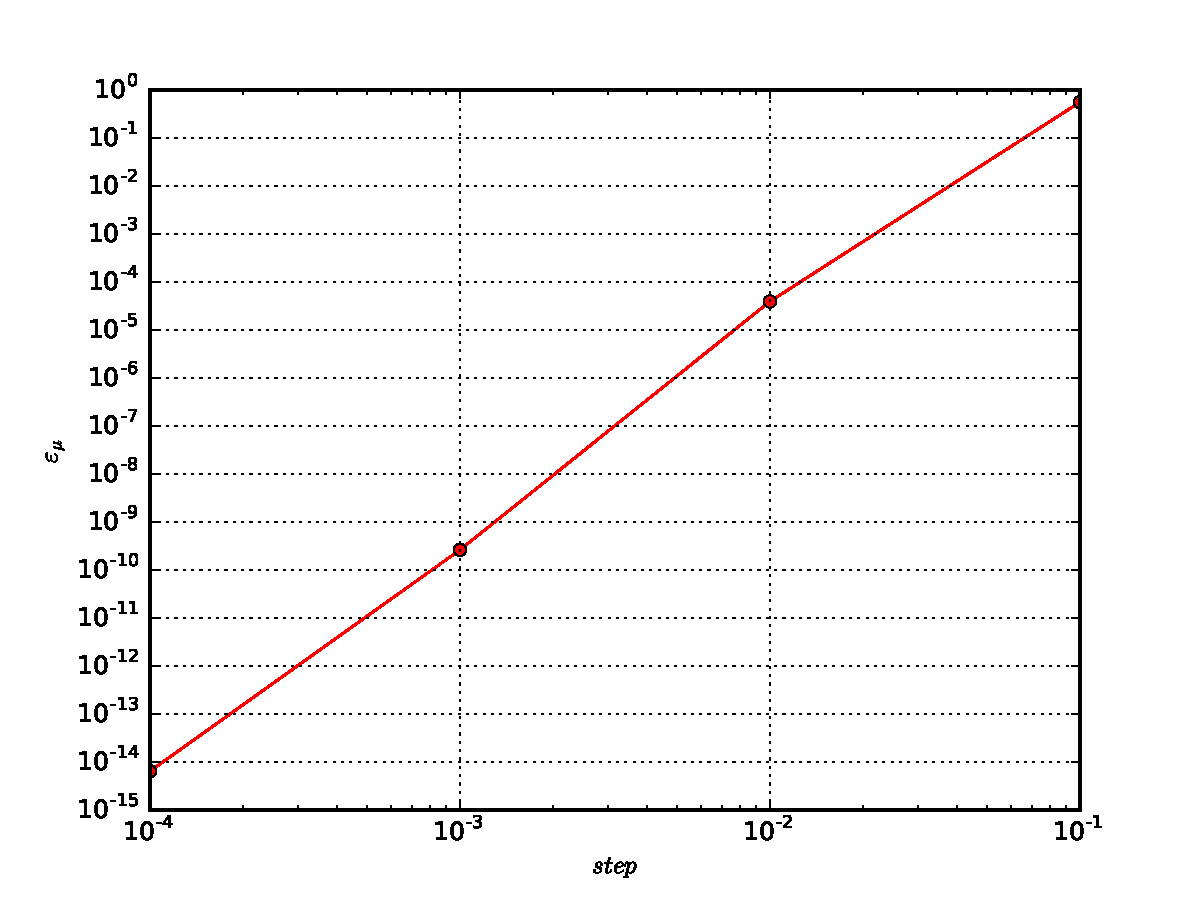
\includegraphics[width=0.75\textwidth]{../pictures/lab5_eigvals_error.pdf}
	\caption{Отклонение модуля собственных чисел матрицы-пропагатора от 1}
	\label{fig:eigvals_error}
\end{figure}

\section{Исходный код}
\lstinputlisting[language=Python, numbers=left]{../scripts/lab5.py}

\end{document}
